\chapter{Optimeringsmetoder} \label{kap:optimeringsmetoder}
\textit{Lasso problemet er et quadratic programming problem med lineære uligheder. 
Flere algoritmer kan løse dette problem grundet konveksiteten.  
I dette kapitel beskrives to af disse algoritmer kaldet coordinate descent og Least Angle Regression (LARS).} \\[4mm]
%
For en model matrix i general position (se definition \ref{defn:general_position}) findes der ikke en eksplicit løsning for lasso estimatoren.
Men som sagt er objektfunktionen af lasso problemet \eqref{eq:2.5} konveks.
For at vise dette kan objektfunktionen skrives som
\begin{align}
f \del{\beta} = g \del{\beta} + h \del{\beta}, \label{eq:opdeling_fkt}
\end{align}
hvor \(g \del{\beta} = \frac{1}{2n} \Vert \y - \X \beta \Vert_2^2\) og \(h \del{\beta} = \lambda \Vert \beta \Vert_1\).
For \(g \del{\beta}\) udregnes Hessematricen
\begin{align*}
\Delta^2 g \del{\beta} = \frac{\partial^2 g }{\partial \beta_i \partial \beta_j} = 2 \X^T \X.
\end{align*}
For enhver vektor \(\ell \in \R^p\) er \(\ell^T \X^T \X \ell > 0\), dvs \(\ell^T \X^T \X \ell \) er positiv semidefinit, hvilket medfører at \(g \del{\beta}\) er konveks.
For ethvert \(\alpha \in \del{0,1}\) og \(\beta\), \(\beta'\) har vi at
\begin{align*}
h \del{\alpha \beta + \del{1+\alpha}\beta'} &= \lambda \Vert \alpha \beta + \del{1+\alpha} \beta' \Vert_1 \\
&\leq \lambda \Vert \alpha \beta \Vert_1 + \lambda \Vert \del{1+\alpha} \beta' \Vert_1 \\
&= \lambda \alpha \Vert \beta \Vert_1 + \lambda \del{1+\alpha} \Vert \beta' \Vert_1 \\
&= \alpha h \del{\beta} + \del{1+\alpha} h \del{\beta'},
\end{align*}
hvilket medfører, at \(h \del{\beta}\) er konveks af definition \ref{defn:konveks}.
Da summen af to konvekse funktioner er konveks, medfører dette konveksiteten af \(f \del{\beta}\). 

Som nævnt i underafsnittet \ref{subsec:udregning_lasso} er \(\ell_1\)-normen \(\sum_{j=1}^p \vert \beta_j \vert\) ikke differentialbel i \(\beta = 0\).
En general egenskab af differentialble konvekse funktioner er, at en første ordens tangent approksimation altid giver en nedre grænse.
Begrebet subgradient er baseret på en generalisering af dette.
Givet en konveks funktion \(f: \ \R^p \rightarrow \R\), siges \(z \in \R^p\) at være en subgradient af \(f\) i \(\beta\) hvis
\begin{align*}
f \del{\beta'} \geq f \del{\beta} + \left\langle z, \beta' - \beta \right\rangle, 
\end{align*}
for alle \(\beta' \in \R^p\).
Geometrisk er subgradient vektoren \(z\) normal til et hyperplan som understøtter ---.
Mængden af alle subgradienter af \(f\) i \(\beta\) kaldes \textit{subdifferential} og betegnes \(\partial f \del{\beta}\).
Når \(f\) er differentialble i \(\beta\), da reduceres subdifferentialet til én vektor, givet ved \(\partial f \del{\beta} = \cbr{\nabla f \del{\beta}}\).
I punkter hvor \(f\) ikke er differentialble, da er subdifferentialet en konveks mængde bestående af alle mulige subgradienter.




\section{Coordinate descent} \label{sec:theory_coordinatedescent}
%Ideen bag coordinat descent er, at optimere en target funktion mht én parameter mens de resterende parametre fastholdes. 
%Vi gennemløber alle parametre iterativ indtil konvergens.
%Coordinate descent er specielt attraktiv for problemer som lasso, som har en simpel lukket løsning for en dimension, men ikke for flere dimensioner.
%
Coordinate descent er en iterativ algoritme, som opdaterer fra \(\tbeta^t\) til \(\tbeta^{t+1}\) ved at vælge én koordinat som opdateres, og da udføres en univariat minimering over denne koordinat.
Hvis koordinat $k$ er valgt i iteration $t$, da er opdateringen givet ved
\begin{align}
\beta_k^{t+1} =\underset{ \beta_k}{\arg \min}  f\del{ \beta_1^t, \beta_2^t, \dots, \beta_{k-1}^t, \beta_k, \beta_{k+1}^t, \dots, \beta_p^t  }, \label{eq:5.36}
\end{align}
hvor $\beta_j^{t+1} = \beta_j^t$ for $j \neq k$. 
Typisk gennemløbes koordinaterne i en forudbestemt rækkefølge.
Dette kan generaliseres til \textit{block coordinate descent}, som anvendes for group lasso, hvor prædiktorerne er opdelt i ikke-overlappende blocks, og da udføres en minimering over en enkelt block for hvert koordinat.

For at algoritmen konvergerer til det globale minimum af en konveks funktion, skal funktionen være kontinuert differentiabel og strengt konveks i hver koordinat. 
Men som nævnt er strafleddet for lasso ikke differentiabel.

For mange optimeringsproblemer kan objektfunktionen dekomponeres
\begin{align}
f(\beta_1, \dots, \beta_p) = g(\beta_1, \dots, \beta_p) + \sum_{j = 1}^p h_j \del{\beta_j}, \label{eq:5.37}
\end{align}
hvor \(g: \R^p \rightarrow \R\) er differentiabel og konveks og \(h_j: \R \rightarrow \R\) er konveks, men ikke nødvendigvis differentiabel.
Bemærk at lasso problemet \eqref{eq:2.5} kan dekomponeres som \eqref{eq:5.37} med \(g \del{\tbeta} =\Vert \y - \X \tbeta \Vert_2^2\) og \(h_j \del{\beta_j} = \lambda \vert \beta_j \vert\).
\citep{Tseng_coordinate} viste, at for enhver konveks funktion \(f\) som kan opdeles som \eqref{eq:5.37}, vil coordinate descent algoritmen \eqref{eq:5.36} konvergere til det globale minimum. 
Nøgleegenskaben bag dette resultat er, at den ikke-differentiable komponent \(h \del{\beta} = \sum_{j=1}^p h_j \del{\beta_j}\), kan opsplittes som summen af funktioner af hver individuel parameter.
Resultatet betyder, at coordinate descent kan bruges til at løse lasso og dens generaliseringer, som beskrives senere i specialet.
Hvis den ikke-differentiable komponent \(h\) ikke kan opsplittes, da kan det ikke garanteres at coordinate descent konvergerer.

%\subsubsection{Lineær regression og lasso}
%Optimalitets betingelserne for lasso problemet \eqref{eq:2.5} er
%\begin{align*}
%-2 \sum_{i=1}^n \del{y_i - \sum_{k=1}^p x_{ik} \beta_k} x_{ij} + \lambda s_j = 0,
%\end{align*}
%hvor \(s_j =\text{sign} \del{\beta_j^*}\) hvis \(\beta_j^* \neq 0\) og \(s_j \in \sbr{-1,1}\) hvis \(\beta_j^* = 0\) for \(j=1, \ldots, p\).
%Coordinate descent algoritmen løser disse ligninger og itererer over \(j=1,2,\ldots,p,1,2, \ldots\).
%Lad os definer det partielle residual \(r_i^{(j)} = y_i - \sum_{k \neq j} x_{ik} \widehat{\beta}_k\), som fjerner nuværende fit fra alle undtaget \(j\)'te prædiktor.
%Da er opdateringen givet ved
%\begin{align*}
%\widehat{\beta}_j = S_\lambda \del{\tilde{\beta}_j},
%\end{align*}
%hvor \(\tilde{\beta}_j\) er koefficienten af en simpel lineær regression af det partial residual på variabel \(j\).
\newpage
\begin{alg} [Coordinate descent for lasso problemet]
\begin{enumerate}
\item Standardisér prædiktorerne \(\x_1, \ldots, \x_p\) og centrér responsvariablen.
Definer en følge af værdier \(\lambda_0 > \lambda_1 > \ldots > \lambda_L\), hvor \(\lambda_0\) vælges, således at \(\widehat{\tbeta}^\text{lasso} \del{\lambda_0} =\mathbf{0}\).
\item For hvert \(\lambda \in \cbr{\lambda_0, \ldots, \lambda_L}\), gentages følgende trin for \(j = 1, \ldots, p\) indtil konvergens:
\begin{itemize}
\item Opskriv lasso problemet \eqref{eq:2.5}
\begin{align*}
\sum_{i=1}^n \del{y_i - \sum_{k \neq j} x_{ik} \widehat{\beta}^\text{lasso}_k - x_{ij} \beta_j}^2 + \lambda \sum_{j = 1}^p \vert \beta_j \vert,
\end{align*}
hvor \(\widehat{\beta}^\text{lasso}_k \del{\lambda}\) er det nuværende estimat for \(\beta_k\) for et given \(\lambda\), hvor \(k \neq j\).
\item Udregn de partielle residualer: \(r_{i}^{(j)} = y_i - \sum_{k \neq j} x_{ik} \widehat{\beta}^\text{lasso}_k \del{\lambda}\) for alle \(i\)
\item Udregn koefficienten af en simpel lineær regression af den partielle residual på \(j\)'te prædiktor: \(\tilde{\beta}_j = \frac{1}{n} \sum_{i=1}^n r_{i}^{(j)} x_{ij}\) 
\item Opdater det nuværende estimat \(\widehat{\beta}^\text{lasso}_j\) ud fra soft-thresholding operatoren
\begin{align}
\widehat{\beta}^\text{lasso}_j \del{\lambda}= S_{\frac{\lambda}{2n}} \del{\tilde{\beta}_j}. \label{eq:update_coordinate}
\end{align}
\end{itemize}
\end{enumerate}
\end{alg}
%
Løsningerne udregnes for en aftagende følge af værdier \(\cbr{\lambda_{\ell}}_{\ell = 0}^L\), hvor \(\lambda_0\) vælges således at \(\widehat{\tbeta} \del{\lambda_0} =\mathbf{0}\). 
Algoritmen udnytter \textit{warm start}, hvilket betyder, at \(\widehat{\tbeta} \del{\lambda_\ell}\) anvendes som begyndelsesværdi for løsningen \(\widehat{\tbeta} \del{\lambda_{\ell + 1}}\), dette fører til en mere stabil algoritme. 
Når \(\widehat{\tbeta} = \mathbf{0}\), har vi, at \(\widehat{\beta}_j\) vil forblive nul hvis \(\frac{1}{n} \left\vert \left\langle \mathbf{x}_j, \mathbf{y} \right\rangle \right\vert < \frac{\lambda}{2n}\). Derfor er \( \lambda_0 = 2 \max_j \left\vert \left\langle \mathbf{x}_j, \mathbf{y} \right\rangle \right\vert\).
Strategien er at vælge en minimum værdi \(\lambda_L = \epsilon \lambda_0\) og konstruere en følge af \(K\) værdier af \(\lambda\), som aftager fra \(\lambda_0\) til \(\lambda_L\) på logskalaen.
Typiske værdier er \(\epsilon = 0.001\) og \(K =100\).

Den beskrevne coordinate descent algoritme er implementeret i \Rlang-pakken \texttt{glmnet}.
Koefficientstierne i figur \ref{fig:diabetes_koef} er fundet ud fra denne algoritme.

\section{LARS}
Først vil vi beskrive LARS algoritmen, hvorefter vi vil introducere en simpel modifikation, som fører til lasso estimater. \\[2mm]
%
I grove træk fungerer algoritmen som følgende. 
Først sættes alle koefficienter lig nul, og vi finder prædiktoren, som er mest korreleret med responsvariablen \(\y\), denne prædiktor betegnes \(x_{j_1}\).
Der udføres en simpel lineær regression af \(\y\) på \(x_{j_1}\), hvoraf vi finder en residualvektor.
%som herefter betragtes som responsvariablen.
Herefter tages det størst mulige step i retningen af denne prædiktor indtil en anden prædiktor, som betegnes \(x_{j_2}\), har samme korrelation med den nuværende residual.
Istedet for at fortsætte langs \(x_{j_1}\) fortsætter LARS i en retning, som er ensvinklet mellem de to prædiktorer, indtil en tredje variabel bliver den mest korreleret mængde.
LARS fortsætter da ensvinklet imellem \(x_{j_1}\), \(x_{j_2}\) og \(x_{j_3}\), dvs langs ``least angle direction'' indtil en fjerde variable medtages, osv.

LARS finder estimaterne \(\widehat{\tmu} = \X \widehat{\tbeta}\) ved at tilføje én prædiktor til modellen i hvert step, således at præcis \(k\) estimater er forskellig fra nul efter \(k\) steps.

Figur \ref{fig:lars} illustrerer algoritmen, hvor $p = 2$ og $\X = \del{\textbf{x}_1 \  \textbf{x}_2}$.
I dette tilfælde afhænger de nuværende korrelationer, givet ved \(\textbf{c}\del{\boldsymbol{\widehat{\mu}}} = \X^T\del{\textbf{y} - \widehat{\boldsymbol{\mu}}}\), kun af projektionen \(\bar{\y}_2\) af \(\y\) på det lineære rum $\mathcal{L} \del{\X}$ udspændt af \(\x_1\) og \(\x_2\), dvs 
\begin{align*}
\textbf{c}\del{\boldsymbol{\widehat{\mu}}} =  \X^T \del{ \bar{\y}_2 - \boldsymbol{\widehat{\mu}}}.
\end{align*}
Algoritmen starter i $\widehat{\boldsymbol{\mu}}_0 = \textbf{0}$.
På figur \ref{fig:lars} ses, at vinklen mellem \(\bar{\y}_2 - \widehat{\boldsymbol{\mu}}_0\) og \(\x_1\) er mindre end vinklen mellem \(\bar{\y}_2 - \widehat{\boldsymbol{\mu}}_0\) og \(\x_2\) og dermed fås \(c_1 \del{\widehat{\boldsymbol{\mu}}_0} > c_2 \del{\widehat{\boldsymbol{\mu}}_0}\).
%\(\bar{\y}_2 - \widehat{\boldsymbol{\mu}}_0\) har en mindre vinkel med \(\x_1\) end \(\x_2\), dvs \(c_1 \del{\widehat{\boldsymbol{\mu}}_0} > c_2 \del{\widehat{\boldsymbol{\mu}}_0}\).
Derfor tilføjer LARS \(\widehat{\boldsymbol{\mu}}_0\) i retningen af \(\x_1\), og vi får
\begin{align*}
\widehat{\tmu}_1 = \widehat{\tmu}_0 + \widehat{\gamma}_1 \x_1,
\end{align*}
hvor stepstørrelsen \(\widehat{\gamma}_1\) vælges, således at korrelationen mellem \(\bar{\y}_2 - \widehat{\tmu}_1\) og \(\x_1\) er lig korrelationen mellem \(\bar{\y}_2 - \widehat{\tmu}_1\) og \(\x_2\).
%  \(\bar{\y}_2 - \widehat{\tmu}_1\) er ligeså korreleret med \(\x_1\) som med \(\x_2\).
Dermed halverer \(\bar{\y}_2 - \widehat{\boldsymbol{\mu}}_1\) vinklen mellem \(\x_1\) og \(\x_2\), således at \(c_1 \del{\widehat{\boldsymbol{\mu}}_1} = c_2 \del{\widehat{\boldsymbol{\mu}}_1}\).
%
\begin{figure}[H]
\centering
\scalebox{0.8}{\begin{tikzpicture}
%\draw [<-] (4,0) node [below] {$\x_1$}-- (-3,0);
\draw [blue] [<-] (1,0) node [below] {$\widehat{\tmu}_1$} -- (-3,0);
\draw [<-] (4,0) node [below] {$\x_1$} -- (1,0);
\filldraw [blue] (1,0) circle (2pt) node [below, black] {$\widehat{\boldsymbol{\mu}}_1$};
\filldraw [green] (-3,0)  circle (2pt) node [below, black]{$\widehat{\boldsymbol{\mu}}_0$};
\draw [dashed] [<-] (5,4) node [above] {$\x_2$} --(1,0);
\draw [<-] (1,4) node [above] {$\x_2$} --(-3,0);

\draw [green] (5,1.66) node [above, black] {$\bar{\y}_2$} -- (-3,0);
\filldraw [green] (5,1.66) circle (2pt);
\draw [blue] [->] (1,0) -- (3, 0.83) node [below, black] {$\mathbf{u}_2$} ;
\draw [green] (3,0.83) -- (5,1.66) ; 

\draw [green] (5,0) node [below] {} -- (4.1,0);
\filldraw [green] (5,0) circle (2pt) ;
\draw (5,0) node [black, below] {$\bar{\y}_1$};
\end{tikzpicture}}
\caption{LARS algoritmen for \(p=2\). \(\bar{\y}_2\) er projektionen af \(\y\) på det lineære underrum \(\mathcal{L} \del{\x_1, \x_2}\).
Algoritmen starter i \(\widehat{\tmu}_0=\mathbf{0}\). Residualvektoren \(\bar{\y}_2 - \widehat{\tmu}_0\) har en større korrelation med \(\x_1\) end \(\x_2\). Næste LARS estimat er \(\widehat{\tmu}_1 = \widehat{\tmu}_0 + \widehat{\gamma}_1 \x_1\), hvor \(\widehat{\gamma}_1\) vælges, således at \(\bar{\y}_2 - \widehat{\tmu}_1\) halverer vinklen mellem \(\x_1\) og \(\x_2\). Næste LARS estimat er \(\widehat{\tmu}_2 = \widehat{\tmu}_1 + \widehat{\gamma}_2 \mathbf{u}_2\), hvor \(\mathbf{u}_2\) er en enhedsvektor, som ligger langs denne halveringslinje.
Der gælder, at \(\widehat{\tmu}_2 = \bar{\y}_2\) for \(p=2\), dette er ikke tilfældet for \(p>2\), som ses på figur \ref{fig:lars2}.
 }\label{fig:lars}
\end{figure}
%
Lad $\mathbf{u}_2$ være enhedsvektoren, som ligger langs denne halveringslinje.
Det næste LARS estimat er dermed
\begin{align*}
\widehat{\boldsymbol{\mu}}_2 = \widehat{\boldsymbol{\mu}}_1+ \widehat{\gamma}_2 \mathbf{u}_2,
\end{align*}
hvor $\widehat{\gamma}_2$ er valgt, således at $\widehat{\boldsymbol{\mu}}_2 = \bar{\textbf{y}}_2$ i dette tilfælde hvor $p = 2$. 
For \(p>2\), da vil stepstørrelsen \(\widehat{\gamma}_2\) være mindre, hvilket fører til en anden ændring af retningen, som illustreres på figur \ref{fig:lars2}.
%
\begin{figure}[H]
\centering
\scalebox{0.8}{\begin{tikzpicture}
\filldraw [green] (-3,0) circle (2pt) node [below, black]{$\widehat{\tmu}_0$};
\draw [<-] (6.8,0) node [below] {$\x_1$} -- (-3,0);
\draw [<-] (1,4) node [above] {$\x_2$} --(-3,0);
\draw [<-] (-5,4) node [above] {$\x_3$} --(-3,0);

\draw [green] (4,0) node [above, black] {$\bar{\y}_1$} -- (-3,0);
\filldraw [green] (4,0) circle (2pt) ;
\draw [blue] (1,0) node [below, black] {$\widehat{\tmu}_1$} -- (-3,0);
\draw [blue] [->] (-3,0) -- (-1.5, 0) node [below, black] {$\mathbf{u}_1$} ;

\draw [green] (6,2.1) node [above, black] {$\bar{\y}_2$} -- (1,0);
\filldraw [green] (6,2.1) circle (2pt) ;
\draw [blue] (4,1.25) node [below, black] {$\widehat{\tmu}_2$} -- (1,0);
\draw [blue] [->] (1,0) -- (2.6, 0.65) node [below, black] {$\mathbf{u}_2$} ;

\draw [green] (5,3.5) node [above, black] {$\bar{\y}_3$} -- (4,1.25);
\filldraw [green] (5,3.5) circle (2pt) ;
\draw [blue] [<-] (4.4,2.2)  -- (4,1.25);
\draw [blue] (4.8,3.1)-- (4.4,2.2);
\draw [blue] [<-] (4.5,3.5) -- (4.8,3.1);
\end{tikzpicture}}
\caption{I hvert step nærmer LARS estimatet \(\hat{\tmu}_k\) sig det tilhørende OLS estimat \(\bar{\y}_k\), men vil aldrig nå det.
 }\label{fig:lars2}
\end{figure}
%
Vi antager, at prædiktorerne \(\x_1, \ldots, \x_p\) er lineært uafhængige.
Lad \(\A\) være en delmængde af indekser \(\cbr{1,\ldots, p}\), og definer matricen
\begin{align}
\X_\A = \del{\dots s_j \x_j \dots}_{j \in \A}, \label{eq:lars_2.4}
\end{align}
hvor $s_j = \pm 1$, således at \(\X_\A\) er en matrix, som består af søjlerne i \(\X\), der er inkluderet i \(\mathcal{A}\) multipliceret \(s_j\).
Lad 
\begin{align}
N_\A = \X_\A^T \X_\A \quad \text{og} \quad A_\A = \del{\mathbf{1}_\A^T N_\A^{-1} \mathbf{1}_\A}^{-1/2}, \label{eq:lars_2.5}
\end{align}
hvor \(\mathbf{1}_\A\) er en vektor af 1-taller med en længde lig antallet af elementer i \(\A\).
Da defineres en såkaldt ``ensvinklet'' vektor
\begin{align}
\mathbf{u}_\A = \X_\A \omega_\A, \quad \text{hvor } \omega_\A = A_\A N_\A^{-1} \mathbf{1}_\A, \label{eq:lars_2.6}
\end{align}
som er en enhedsvektor, der gør vinkler mellem søjlerne i \(\X_\A\) lige store, dvs
%der resulterer i lige store vinkler der er mindre end \(90^0\), med søjlerne i \(\X_\A\), dvs
\begin{align}
\X_\A^T \mathbf{u}_\A = A_\A \mathbf{1}_\A \quad \text{og} \quad \Vert \mathbf{u}_\A \Vert_2^2 = 1. \label{eq:lars_2.7}
\end{align}
Herefter kan vi give en fyldestgørende beskrivelse af LARS algoritmen.
%
\begin{alg} [LARS algoritmen]
\begin{enumerate}
\item Standardisere prædiktorerne og centre responsvariablen. 
Start med \(\widehat{\boldsymbol{\mu}}_0 = \mathbf{0}\), \(\widehat{\mathbf{c}} = \X^T \y\), og \(\A = \emptyset\).
\item Find prædiktoren \(\tx_j\) som er mest korreleret med \(\y\). Definer den aktive mængde \(\A = \cbr{j}\).
\item Gentag følgende indtil alle prædiktorer er indeholdt i den aktive mængde:
\begin{itemize}
\item Antag \(\widehat{\boldsymbol{\mu}}_\A\) er det nuværende LARS estimat og at
\begin{align}
\widehat{\mathbf{c}} = \X^T \del{\y - \widehat{\boldsymbol{\mu}}_\A}, \label{eq:lars_2.8}
\end{align} 
er vektoren af nuværende korrelationer.
Den aktive mængde \(\A\) er en mængde af indekser svarende til prædiktorer med størst absolut nuværende korrelationer
\begin{align}
\widehat{C} = \max_j \cbr{\abs{\widehat{c}_j}} \quad \text{og} \quad \A= \cbr{j: \ \abs{ \widehat{c}_j} = \widehat{C}}. \label{eq:lars_2.9}
\end{align}
Lad 
\begin{align*}
s_j = \text{sign} \cbr{\widehat{c}_j}, \quad j \in \A,
\end{align*}
da udregnes \(\X_\A\), \(A_\A\) og \(\mathbf{u}_\A\) som i \eqref{eq:lars_2.4}-\eqref{eq:lars_2.6} samt
\begin{align*}
\mathbf{a} = \X^T \mathbf{u}_\A.
\end{align*}
\item Opdatere \(\widehat{\boldsymbol{\mu}}_\A\) til
\begin{align}
\widehat{\boldsymbol{\mu}}_{\A_+} = \widehat{\boldsymbol{\mu}}_\A + \widehat{\gamma} \mathbf{u}_\A, \label{eq:lars_2.12}
\end{align}
hvor 
\begin{align}
\widehat{\gamma} = \min_{j \in \A^c}^+ \cbr{ \frac{\widehat{C}- \widehat{c}_j}{A_\A - a_j} , \frac{\widehat{C} + \widehat{c}_j}{A_\A + a_j}}, \label{eq:lars_2.13}
\end{align}
og hvor \(\min^+\) indikerer, at minimum kun tages over de positive komponenter indenfor valget af \(j\) i \eqref{eq:lars_2.13}.
\item Sæt \(\A = \A \cup \cbr{\widehat{j}}\), hvor \(\widehat{j}\) er minimeringsindekset i \eqref{eq:lars_2.13}.
\end{itemize}
\end{enumerate}
\end{alg}
%
Formlerne \eqref{eq:lars_2.12} og \eqref{eq:lars_2.13} har følgende fortolkning.
Definer
\begin{align}
\tmu \del{\gamma} = \widehat{\tmu}_\A + \gamma \mathbf{u}_\A, \label{eq:lars_2.14}
\end{align}
for \(\gamma > 0\), således at den nuværende korrelation er givet ved
\begin{align}
c_j \del{\gamma} = \x_j^T \del{\y - \tmu \del{\gamma}} = \widehat{c}_j - \gamma a_j. \label{eq:lars_2.15}
\end{align}
For \(j \in \A\) giver \eqref{eq:lars_2.7}-\eqref{eq:lars_2.9} at
\begin{align}
\abs{c_j \del{\gamma}} = \widehat{C} - \gamma A_\A,\label{eq:lars_2.16}
\end{align}
som viser, at alle af de maksimale absolutte nuværende korrelationer falder ligeligt.
For \(j \in \A^C\), viser \eqref{eq:lars_2.15} og \eqref{eq:lars_2.16} at \(c_j \del{\gamma}\) er lig den maksimale værdi i \(\gamma = \frac{\widehat{C} - \widehat{c}_j}{A_\A - a_j}\).
Derfor er \(\widehat{\gamma}\) i \eqref{eq:lars_2.13} den mindst positive værdi af \(\gamma\), således at et nyt indeks \(\widehat{j}\) tilføjes til den aktive mængde.
\(\widehat{j}\) er minimeringsindekset i \eqref{eq:lars_2.13} og den nye aktive mængde \(\A_+\) er \(\A \cup \cbr{\widehat{j}}\) og den nye maksimum absolut korrelation er \(\widehat{C}_+ = \widehat{C}- \widehat{\gamma} A_\A\).
%
%\begin{figure}[H]
%\centering
%\scalebox{0.6}{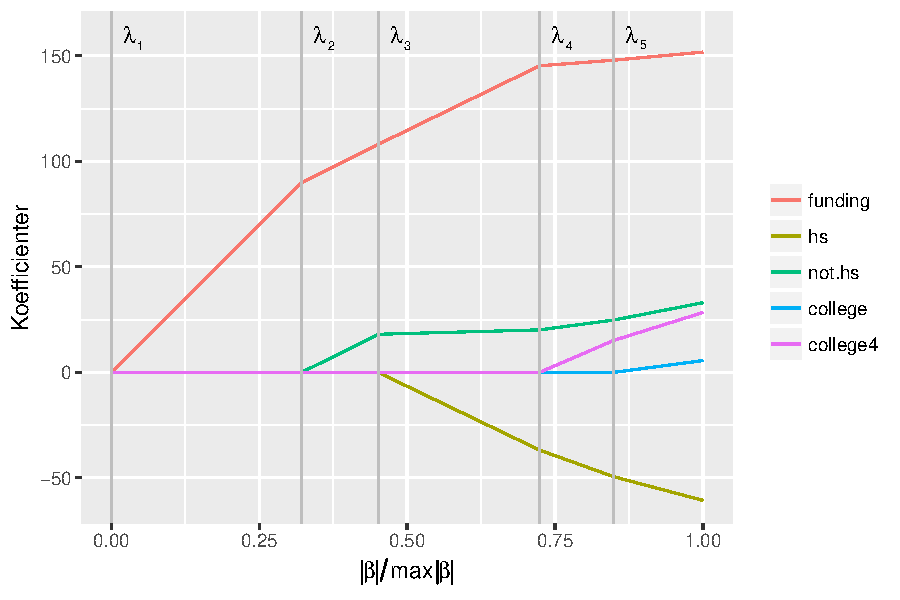
\includegraphics{fig/img/crime_lars_lasso.pdf}}
%\caption{Koefficientstierne udregnet med LARS imod fraktion af \(\ell_1\) norm for crime data.} \label{fig:crime_lar}
%\end{figure}
%%
%Figur \ref{fig:crime_lar} illustrerer lars estimaterne som funktion af shrinkage for crime data.
%Af figuren kan vi aflæse rækkefølgen, hvori variablerne medtages i modellen.
%For \(s=0\), er der ingen variable i modellen, som ses til ventre.
%Hvis vi bevæger os mod højre ses at den første variabel som medtages i modellen er variabel 1 (\texttt{funding}), efterfulgt at variabel 3 (\texttt{not.hs}), derefter 2 (\texttt{hs}), variabel 5 (\texttt{college4}) og til slut variabel 4 (\texttt{college}). 
%Algoritmen kræver \(p=5\) steps.
%
%Højre figur viser de absolutte nuværende korrelationer
%\begin{align*}
%\abs{\widehat{c}_{kj}} = \abs{\x_j^T \del{\y - \widehat{\tmu}_{k-1}}},
%\end{align*}
%for \(j = 1, \ldots, 5\) som en funktion af LARS step \(k\).
%Den maksimale korrelation
%\begin{align*}
%\widehat{C}_k = \max \cbr{\abs{\widehat{c}_{kj}}} = \widehat{C}_{k-1} - \widehat{\gamma}_{k-1} A_{k-1},
%\end{align*}
%aftager med \(k\) som forventet.
%I hvert step tilføjes en ny variabel \(j\) til den aktive mængde, derfor har vi, at \(\abs{\widehat{c}_{kj}} = \widehat{C}_k\).
%Fortegnet \(s_j\) af hver \(\x_j\) i \eqref{eq:lars_2.4} forbliver konstant, da den aktive mængde kun stiger.

For LARS algoritmen kræves blot \(p\) steps for at finde den fulde løsning.
De beregnings mæssige omkostninger for LARS algoritmen er af samme orden som løsningen af OLS med \(p\) prædiktorer.


\subsection{Lasso modifikation} \label{subsec:lasso_modifikation}
I dette afsnit beskrives en simpel modifikation af LARS algoritmen, således at den giver lasso estimater.
Lad \(\widehat{\tbeta}^\text{lasso}\) være løsningen til lasso problemet \eqref{eq:2.5} med \(\widehat{\tmu}^\text{lasso} = \X \widehat{\tbeta}^\text{lasso}\).
Da kan det vises, at fortegnet af enhver ikke-nul koefficient \(\widehat{\beta}_j\) og fortegnet \(s_j\) af den nuværende korrelation \(\widehat{c}_j = \x_j^T \del{\y - \widehat{\tmu}}\) må stemmes overens
\begin{align}
\text{sign} \del{\widehat{\beta}_j } = \text{sign} \del{\widehat{c}_j } = s_j, \quad j \in \A. \label{eq:lars_3.1}
\end{align}
%
%\begin{lem}
%For \(\widehat{\beta}^\text{lasso}\) må der gælder, at
%\begin{align*}
%\widehat{c}_j = \widehat{C} \cdot \text{sign} \del{\widehat{\beta}_j},
%\end{align*}
%hvor \(\widehat{c}_j = \x_j^T \del{\y - \widehat{\tmu}}= \x_j^T \del{\y - \X \widehat{\beta}}\).
%Dette medfører, at
%\begin{align}
%\text{sign} \del{\widehat{\beta}_j } = \text{sign} \del{\widehat{c}_j }, \quad j \in \A \label{eq:lars_5.29}
%\end{align}
%\end{lem}
%
Denne restriktion er ikke inkluderet i LARS algoritmen, men kan nemt modificeret hertil. 
Antag vi netop har fuldendt et LARS step, som har givet en ny aktive mængde \(\A\) som i \eqref{eq:lars_2.9}, og at det tilhørende LARS estimat \(\widehat{\tmu}_\A\) svarer til en lasso løsningen \(\widehat{\tmu}^\text{lasso} = \X \widehat{\tbeta}^\text{lasso}\).
Lad
\begin{align*}
\omega_\A = A_\A N_\A^{-1} \mathbf{1}_\A,
\end{align*}
være en vektor med længde lig antallet af elementer i \(\A\) og definer en \(p \times 1\) vektor
\begin{align*}
\widehat{\mathbf{d}} = \begin{cases}
s_j \omega_{\A_j}, &\text{hvis } j \in \A, \\
0, & \text{ellers}.
\end{cases}
\end{align*}
Hvis vi bevæger os i den positive \(\gamma\) retning langs LARS linjen \eqref{eq:lars_2.14}, ser vi, at
\begin{align*}
\tmu \del{\gamma} = \X \tbeta \del{\gamma}, \quad \text{hvor } \beta_j \del{\gamma} = \widehat{\beta}_j + \gamma \widehat{d}_j
\end{align*}
for \(j \in \A\).
Derfor vil \(\beta_j \del{\gamma}\) ændre fortegn i
\begin{align*}
\gamma_j = -\frac{\widehat{\beta}_j}{\widehat{d}_j},
\end{align*}
den første af sådan en ændring kommer i
\begin{align*}
\tilde{\gamma} = \min_{\gamma_j > 0} \cbr{\gamma_j},
\end{align*}
for prædiktor \(\x_{\tilde{j}}\).
Hvis der ikke findes en \(\gamma_j > 0\), da er \(\tilde{\gamma}=\infty\) per definition.

Hvis \(\tilde{\gamma} < \widehat{\gamma}\), da kan \(\beta_{\tilde{j}} \del{\gamma}\) ikke være lasso løsningen for \(\gamma > \tilde{\gamma}\), da restriktionen \eqref{eq:lars_3.1} ikke er opfyldt, eftersom \(\beta_{\tilde{j}} \del{\gamma}\) har ændret fortegn, mens \(c_{\tilde{j}}\) ikke har.
Der gælder, at \(c_{\tilde{j}}\) ikke kan ændre fortegn indenfor ét LARS step da \(\abs{c_{\tilde{j}} \del{\gamma}} = \widehat{C} - \gamma A_\A> 0\) af \eqref{eq:lars_2.16}. \\[2mm]
%
\textbf{Lasso modifikation} \\
Hvis \(\tilde{\gamma} < \widehat{\gamma}\), stop det igangværende LARS step i \(\gamma = \tilde{\gamma}\) og fjern \(\tilde{j}\) fra udregningen af den næste ensvinklet retning.
Dvs
\begin{align*}
\widehat{\tmu}_{\A_+} = \widehat{\tmu}_\A + \tilde{\gamma} \mathbf{u}_\A \quad \text{og} \quad \A_+ = \A - \cbr{\tilde{j}},
\end{align*}
istedet for \eqref{eq:lars_2.12}.

LARS algoritmen med lasso modifikationen tillader den aktive mængde \(\A\) at aftage.
Antallet er steps i LARS algoritmen med lasso modifikationen er dermed større end \(p\).


Lad os opsummere nogle egenskaber af lasso stien.
Stien \(\widehat{\tbeta}^\text{lasso} \del{\lambda}\) er en kontinuert og stykvis lineære funktion af \(\lambda\) med knuder i \(\lambda_1 \geq \lambda_2 \geq \cdots \geq \lambda_r \geq 0\).
I \(\lambda = \infty\) har løsningen \(\widehat{\tbeta}^\text{lasso} \del{\infty}\) ingen aktive variable, dvs \(\A = \emptyset\). 
Vi aftager \(\lambda\) og da markerer hver knude \(\lambda_k\) tilføjelsen eller fjernelsen af en variabel i den nuværende aktive mængde.
Derfor er den aktive mængde og fortegnene af de aktive variable konstant mellem knuderne.

Figur \ref{fig:diabetes_lars} illustrerer koefficientstierne for LARS algoritmen uden og med lasso modifikationen som funktion af fraktion af \(\ell_1\)-norm for diabetes data.
Af figuren kan vi aflæse rækkefølgen, hvori variablerne medtages i modellen.
For LARS algoritmen uden lasso modifikationen udføres 10 steps, mens LARS algoritmen med lasso modifikationen udfører 12 steps.
De 2 ekstra steps som LARS algoritmen med lasso modifikationen udfører kommer af, at variablen \texttt{hdl} fjernes og tilføjes igen i henholdsvis step 11 og 12.

\imgfigh{diabetes_lars.pdf}{0.9}{Koefficientstierne for LARS algoritmen uden og med lasso modifikationen som funktion af fraktion af \(\ell_1\)-normen for diabetes data.}{diabetes_lars}
%

%\subsection{Frihedsgrader og \(C_p\) estimater}
%
%
%
%
%
%LARS har følgende fordele.
%En af dem er, at den giver en ranking af prædiktorer når der bliver tilføjet andre prædiktorer, som ikke er tilfældet med hard treshold. 
%En anden fordel er at algoritmen undgår streng korrelerede prædiktorer, hvis en af de korrelerede prædiktorer allerede er inkluderet, siden at den nye residual vil have lav korrelation med variabler, som er streng korrelerede variabler, som allerede er inkluderet. 
%Derudover er LARS algoritmen ikke er 'greedy', som forward regression, fordi den udnytter en god retning til dens maksimum . 


